\section{Introduction}
\label{sec:intro}

This study focuses on a particular type of Internet censorship called {\em
network-based Internet censorship}, i.e, the impairing or blocking of access to
online content and service {\em intentionally} by the network, a {\em third
party} between the user host and the online content and service
provider~\cite{aceto_internet_2015}, where an example of the online content can
be a blog post on the Web~\cite{zhu2013velocity} and that of the service can be
the Virtual Private Network (VPN) service~\cite{xue280012}.
Figure~\ref{fig:nicensor} illustrates this concept. This type of censorship
needs the control of neither the user hosts and applications nor the content and
service providers.  Rather it requires the access to the network components, such
as, routers and DNS servers between the user hosts and the content and service
providers. It is prevalent among those, such as a state actor, who seek to
block or impair access to politically, culturally, or religiously sensitive content
hosted on a server within or out of its jurisdiction without a need to tamper
with  the user hosts, the user applications, and the content servers.  

The network-based Internet censorship can lead to network
outages~\cite{dainotti2011analysis}.  Differentiating the censorship events
from other types of outages can thus benefit the design and implementation of
Internet network architecture, protocols, and
systems~\cite{aceto2018comprehensive, aceto_internet_2015}.  Understanding the
censorship mechanism can also help develop circumvention
techniques~\cite{winter2012great, chai2019importance, satija2021blindtls}.

Aside from these technical perspectives, there have been pursuits to gauge its
social, political, cultural, and religious
implications~\cite{shishkina2018internet, meserve2018google,
chen2000pornography}. These works reveal the complexity and the intricacy of Internet censorship, which sometimes challenges conventional wisdom
given its prevalence among countries, polities, cultures, and religions 
of a great spectrum~\cite{aryan2013internet, nabi2013anatomy, singh2017characterizing,
yadav2018light, ng2018detecting,
meserve2018google, bock2021even, padmanabhan2021multi, ververis2021understanding}.

\begin{figure}[!htbp]
	\centering
	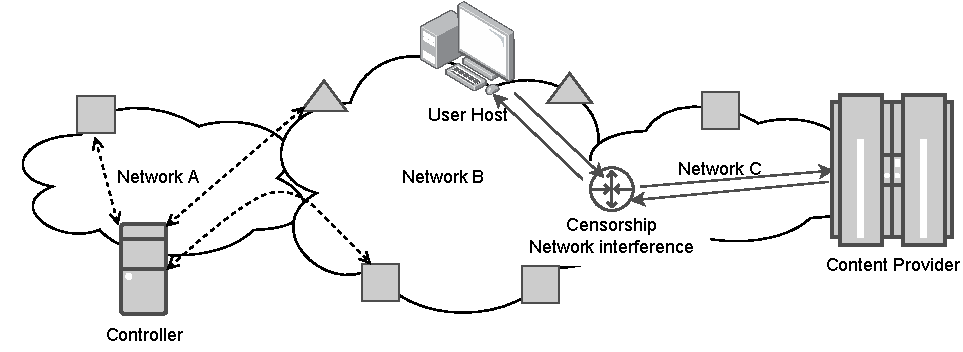
\includegraphics[width=0.9\columnwidth]{figures/censorship.pdf}
	\caption{Network-based Internet censorship and measurement. Network-based
	Internet censorship takes place at neither the user host (or the application
	on the host) nor the content provider. To gauge such censorship, a measurement
	platform sets up vantage points, depicted as squares and triangles in the
	figure. The controller of the platform instructs the vantage point to
	send a network request to the content server or sends a request appearing
	from the vantage point to the content server. Although the existing platforms
	adopt more complex methods, a straightforward method to detect censorship, e.g., whether Network
	B censors a network request is to compare the network traces from multiple
	vantage points. Following that, we can design a fingerprint for the network
	trace for the censored vantage point and the content provider.} 
	\label{fig:nicensor}
\end{figure}

In order to study censorship prevalence and mechanisms systematically, to understand this global phenomenon,
to improve the Internet infrastructure given
the prevalence of it, 
prior efforts have led to
the design, implementation, and deployment of large scale Internet measurement
platforms.  
Internet censorship
manifests as a network reachability problem, i.e., the users are unable to
access the content or the service, or are accessing the content or the service
at a severely degraded quality of service. These platforms are designed to collect
network measurement data about network reachability, 
and further, to detect Internet censorship events from the
reachability data~\cite{sundara_raman_censored_2020, niaki2020iclab,
filasto2012ooni}.
As shown in Figure~\ref{fig:nicensor}, these measurement platforms typically
set up vantage points, strategically or sometimes opportunistically selected
monitoring hosts on the Internet. The platforms typically have controller hosts
(that the platforms may name differently)
and the controllers have network requests sent to the content providers from or
appearing to originate from the vantage points. 

These measurement platforms produce a large amount of network
reachability data~\cite{sundara_raman_censored_2020, niaki2020iclab}.  There
are challenges to detecting censorship events from the reachability data, such as,
the platforms must process the amount of data, and they also need to find a way
to infer whether the reachability problem is intentional to differentiate a
censorship event from an ordinary network outage.  These works generally rely on a
rule-based approach to detect censorship, such as, by matching the measurement
data to censorship fingerprints that are usually purposefully designed regular
expressions~\cite{sundara_raman_censored_2020, niaki2020iclab}. The rule-based
approach has several advantages, such as, it is computationally efficient to
execute a rule, and a carefully designed rule is also unlikely to have a false
detection. However, the rule-based approach has several disadvantages. First,
it requires significant technical expertise.  Second, it is laborious to add
new rules.  Third, it cannot detect any Internet censorship not described by
existing rules. 

Machine learning-based approaches have found applications in software and
system quality assurance and security~\cite{qiao2020deep, lin2020software}.
An improvement over the rule-based approaches where the rules are pre-defined by human
experts manually, the learning-based approaches automatically learn ``rules''
or ``patterns'' in the relevant data. As a result, they can not only offer
better predictive performance than the rule-based systems, but also reduce
human efforts required to design rules for the rule-base systems.
Learning-based approaches are making inroads in both the design of censorship
mechanisms and the data analysis and detection of
censorship~\cite{gao2021machine, li2015predicting}.  Thus far, for
network-based Internet censorship detection, most prior work uses machine
learning algorithms in a semi-automated fashion. For instance, clustering
algorithms are used to group {\em block pages}, notices that content providers
respond to the users to explain the unavailability of requested
content~\cite{jones2014automated}.  A necessary condition to the learning-based
approaches (including clustering) is to express the network reachability data in
a form, i.e., a representation of data, suitable for machine learning
algorithms. This requires us to decide how we extract and represent features
from the data. One approach is to borrow features from natural language
processing, such as, to use features like page length and
term-frequency~\cite{jones2014automated, niaki2020iclab}.  Another is to borrow
approaches from image recognition, such as, to extract feature representations
as screenshots of block pages using ResNet50, a pre-trained convolutional deep
neural network~\cite{raman_measuring_2020}.

Limitations of the prior learning-based approaches for network-based Internet
censorship are two. First, the simple features like page length and
term-frequency do not sufficiently capture nuances in the network reachability
data, e.g., block pages, which results in a high false positive
rates~\cite{yadav2018light}. Second, the prior work primarily uses the learning
algorithms to aid the censorship detection rule design. One example is
FilterMap~\cite{raman_measuring_2020}.  It extracts feature representations from
screenshots of block pages using ResNet50 and clusters block pages into
approximately 200 groups of block pages.  Following this, the researchers
manually design detection rules (signatures of block pages) by examining each
group of block pages. Another example is ICLab~\cite{niaki2020iclab}.  It
computes the term-frequencies of HTML tags and the Locality Sensitive Hashing
index of the text in block pages, produces 48 block page clusters that are
similar either in HTML structures or in page text.  Again, the researchers
manually design new signatures for these clusters in the form of regular expressions. 

Despite these limitations, the prior work has led to the creation of hundreds
of network-based censorship fingerprints in the form of regular expressions and
discovered new censorship events~\cite{niaki2020iclab,
sundara_raman_censored_2020}. In addition, the work also results in the
accumulation of a large amount of reachability data labeled with censorship
types according to the signatures. Taking advantage of these and motivated
by the recent development in deep learning, we present and evaluate a 
censorship detection approach that is built upon well-known deep learning
techniques. The contributions of this work are as follows: 
\begin{enumerate}
	\item The work results in an ``end-to-end'' censorship detection system
		that automates the entire process of censorship detection.  On one
		end, the system automatically learns latent features from network
		reachability data records, which yields feature
		representations of the records. On the other end, from the feature
		presentations, we determine whether a network reachability problem is a
		censorship event via a classification model. The system therefore
		eliminates the need manually to design machine learning features and
		reduces the manual effort to detect new censorship events.  

	\item The network reachability data contains structures and
		pieces of some data elements appear in a particular order. Observing the
		characteristics of the data, we design the feature presentation learning 
		model to be a sequence-to-sequence model adapted from natural language processing. 

	\item The proposed classification model is a supervised learning model. Supervised
		learning models require a large set of labeled data to train, e.g., a
		known set of network measurement records that are labeled as censored or uncensored.  Our
		results show that the proposed supervised learning models trained using
		the block pages labeled by known censorship fingerprints 
		can recognize both known and new censorship
		events.  As a result, we hypothesize that there is additional information
		in the labeled block pages beyond what the signatures capture. 

	\item To evaluate the above end-to-end censorship detection approach and to 
		explore the design space, we design an alternative detection approach 
		that treats network reachability data records as gray-scale images
		and train a state-of-the-art deep learning image classification 
		model to recognize the images as
		censored or not. To compare the two proposed approaches, 
		we process a large collection of Censored Planet block page records.
		The end-to-end approach appears to have an advantage over the
		alternative due in part to the sequence-to-sequence feature representation
		learning.

	\item This work also results in a library of Python scripts that can be used
		for replication and future research. The authors make this library
		publicly available. 
\end{enumerate}

We structure the rest of this article as follows. To situate the proposed work,
we discuss related work in Section~\ref{sec:related}. We introduce our
proposal, the latent feature representation based approach and the image-based
alternative in Section~\ref{sec:design}. In Section~\ref{sec:eval}, we evaluate 
the proposed approaches. Our work isn't without limitations.
We dedicate Section~\ref{sec:threats} to a discussion of the limitations and
the threats to validity. Finally, we conclude this work in
Section~\ref{sec:summary}.




